\documentclass{beamer}
%\usepackage{beamerthemeshadow}
\usetheme{Warsaw}
\usepackage{latexsym,amsbsy,amsopn,amstext,xcolor,multicol,amsmath}
\usepackage{amssymb,graphicx,wrapfig,fancybox}
\usepackage{pgf,pgfarrows,pgfnodes,pgfautomata,pgfheaps,pgfshade}
\usepackage{booktabs}
\usepackage{subfloat}
\usepackage{}
\usecolortheme{}
\graphicspath{{figures/}}

\begin{document}

\title{Group Report}
\subtitle{}
\author{Ma Hsuning}
\institute{physics of NKU}
\date{\today}
\frame{\titlepage}

\section{Introduction}
\subsection{}
\begin{frame}{Introduction}
\begin{itemized}
\item What Do We Do in the Past Two Weeks
\bigskip
Choose from at least two charged tracks, identify one of them as $K$, while another as $\pi$.
Check the invariant mass of those two charged tracks and the number of the good charged tracks.
\end{itemized}
\end{frame}

\section{Works Been Done}
\subsection{}

\begin{frame}{Works Been Being Done}
\begin{itemized}
\item Particle Identification
We identify charged tracks of $K$ and $\pi$ via pid, and restrict the condition to $n_{K} * n_{\pi} >=1$.
\end{itemized}
\end{frame}

\begin{frame}{Raw Results Been Acquired}
   
   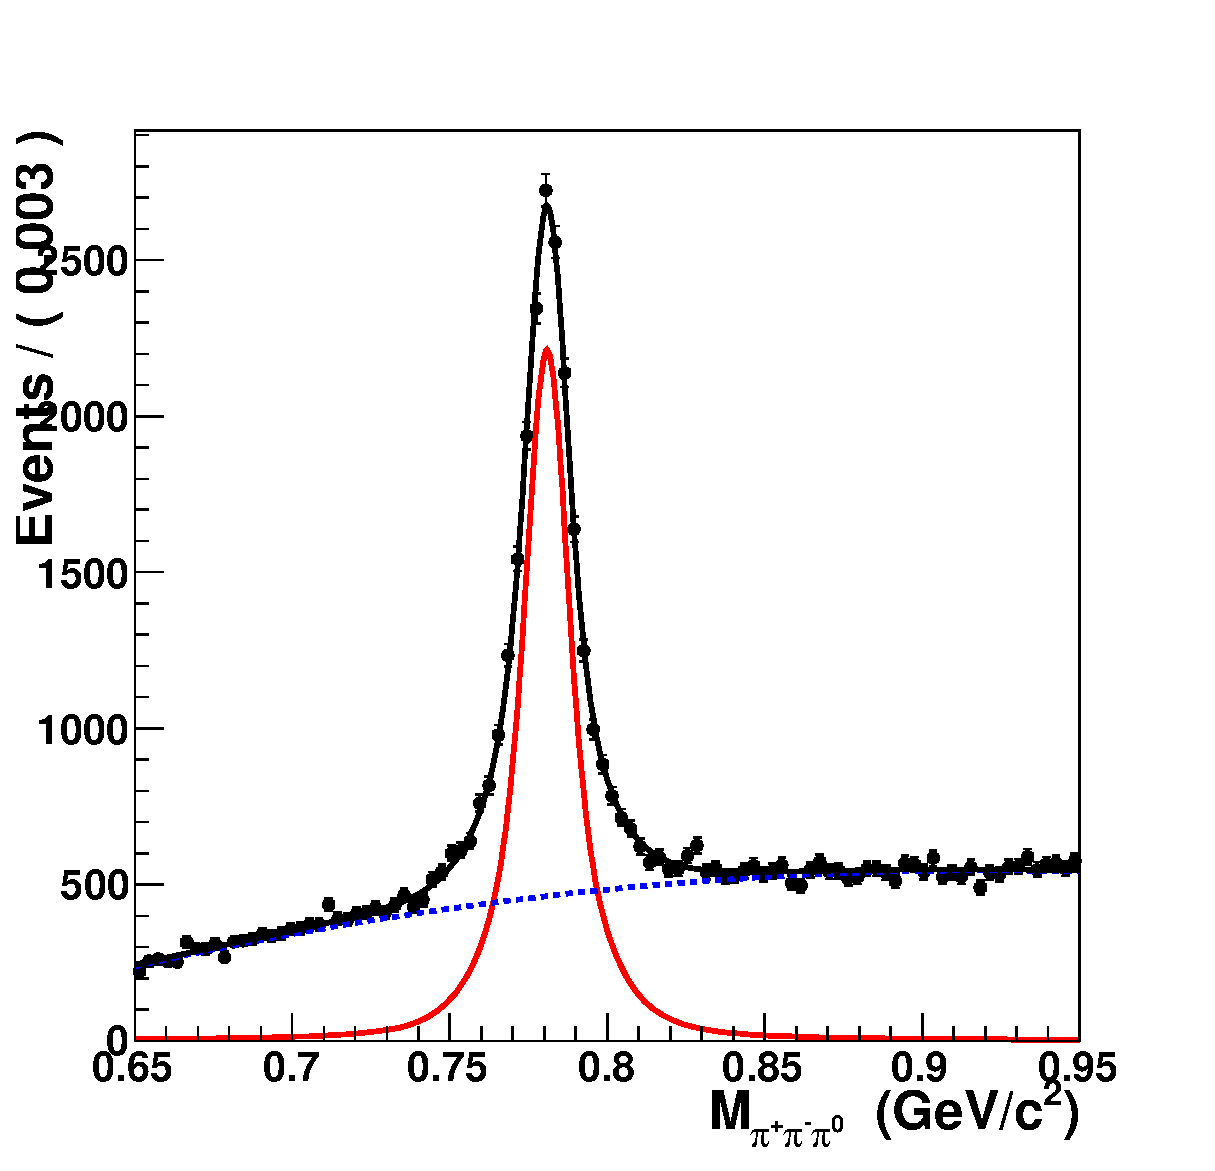
\includegraphics[width=0.8\textwidth]{graphics/signal.eps}
\end{frame}
\section{Works To Be Done}
\end{document}
